\item Sobre la homogeneidad y aditividad de las transformaciones lineales.
    \begin{enumerate}
        \item Dar un ejemplo de una función $f:\R^2\to\R$ tal que \[f(\alpha v)=\alpha f(v)\quad\forall v\in\R^2,\alpha\in\R\] pero que $f$ no sea lineal.
            \begin{mdframed}[style=s]
                Propongo \[f(x,y)=\sqrt[3]{x^2y}\]
                cuya gráfica se muestra en la Figura 2. Dado un $v\in\R^2,\alpha\in\R$
                \begin{align*}
                    f(\alpha v)&=f(\alpha(x,y))\\
                    &=f(\alpha x,\alpha y)\\
                    &=\sqrt[3]{(\alpha x)^2\alpha y}\\
                    &=\sqrt[3]{\alpha^3x^2y}\\
                    &=\alpha\sqrt[3]{x^2y}\\
                    &=\alpha f(x,y)\\
                    &=\alpha f(v)
                \end{align*}
                A pesar de que cumple homogeneidad, no cumple aditividad ya que por ejemplo \[f((0,1)+(1,0))=1\neq f(0,1)+f(1,0)=0\]
                \begin{center}
                    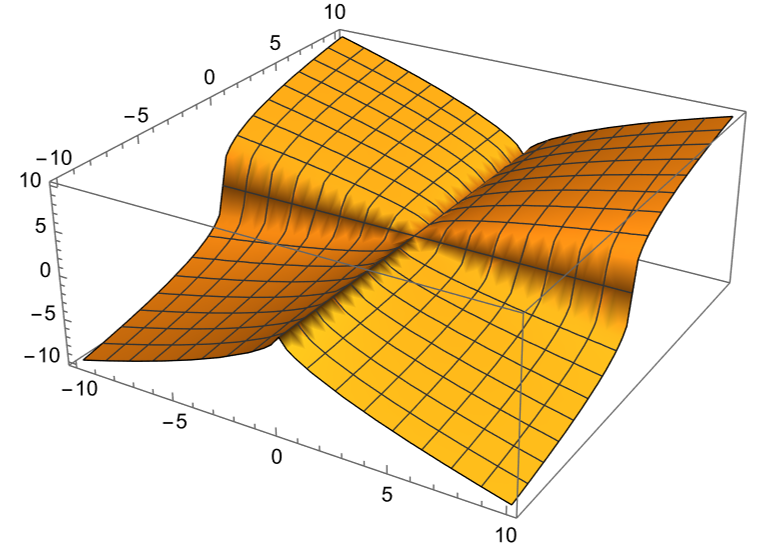
\includegraphics[width=0.4\textwidth]{img/ej10a.png}\\
                    Figura 2. Gráfico de $f(x,y)=\sqrt[3]{x^2y}$ con rectas contenidas.
                \end{center}
                Quizás una manera de visualizar la homogeneidad sea con las rectas de la Figura 2. Al fijar un $v$, por ejemplo el $(1,2)$, al ser multiplicado por un escalar me dará un múltiplo de $v$. Como $v\in\R^2$, la multiplicación por escalar me genera una recta en el plano $z=0$. Entonces si \[f(\alpha v)=\alpha f(v)\quad\forall v\in\R^2,\alpha\in\R\]
                al duplicar el vector $v$, se duplica su imagen, si lo triplico, la imagen también. Es decir, la imagen tiene un incremento constante. Esto se traduce a que la imagen de los puntos de una recta, son una recta. Y como esto sucede con todos los puntos de $\R^2$, se podría decir que la imagen es la unión de las rectas con parametrización:\[\sigma(t)=\left\{\begin{matrix}
                    at\\bt\\\sqrt[3]{(at)^2bt}
                \end{matrix}\right\}\quad a,b\text{ reales fijos},t\in[-\infty,\infty]\]
                En la Figura 3 se observan como un conjunto de estas rectas se aproxima a la función.
                \begin{center}
                    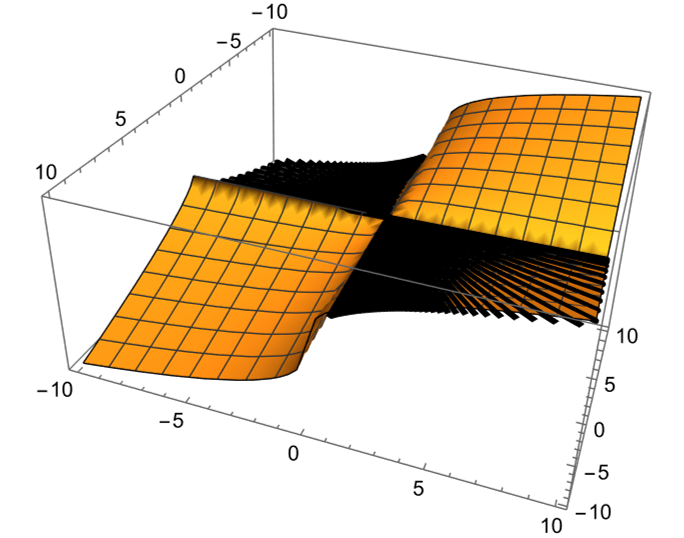
\includegraphics[width=0.4\textwidth]{img/ej10a2.png}\\
                    Figura 3. Gráfico de $f(x,y)=\sqrt[3]{x^2y}$ con múltiples rectas.
                \end{center}
            \end{mdframed}
        \item Dar un ejemplo de una función $g:\C\to\C$ tal que\[g(u+v)=g(u)+g(v)\quad\forall u,v\in\C\] pero que $g$ no sea lineal.
            \begin{mdframed}[style=s]
                La función del ejercicio 8d) cumple con esta condición. 
            \end{mdframed}
    \end{enumerate}